\documentclass[11pt,reqno]{amsart}

\usepackage{amsmath,amssymb,amsthm}
\usepackage{graphicx}
\usepackage[colorlinks=true,allcolors=blue]{hyperref}

\newtheorem{theorem}{Theorem}[section]
\newtheorem{lemma}[theorem]{Lemma}
\newtheorem{proposition}[theorem]{Proposition}
\newtheorem{corollary}[theorem]{Corollary}
\newtheorem{conjecture}[theorem]{Conjecture}
\theoremstyle{definition}
\newtheorem{definition}[theorem]{Definition}
\theoremstyle{remark}
\newtheorem{remark}[theorem]{Remark}

\newcommand{\R}{\mathbb{R}}
\newcommand{\Op}{\mathcal{O}}
\newcommand{\norm}[1]{\lVert #1\rVert}
\newcommand{\ip}[2]{\langle #1,\,#2\rangle}

\begin{document}

\title[Exact fiber analysis of kinetic-balance pollution]{Exact fiber
analysis of kinetic-balance spectral pollution for the radial Dirac
operator}

\author{C.~D.~Reinoso}
\address{Facultad de Ciencias, Escuela Superior Polit\'ecnica de
Chimborazo (ESPOCH), Riobamba, Ecuador}
\email{cesardanielrrch@gmail.com}

\date{\today}

\begin{abstract}
Galerkin discretizations of the radial Dirac operator are notorious for
spectral pollution: spurious eigenvalues inside the essential gap that
kinetic-balance prescriptions are designed to suppress. We show that for
the discretized free operator this phenomenon admits an exact,
completely elementary analysis. The free Dirac matrix built on any
scalar basis decomposes into two-dimensional fibers indexed by the
singular values of the coupling matrix, and on each fiber the sector
leakage of the balanced, split and anti-balanced trial families is an
explicit algebraic function of the dimensionless fiber parameter
$t=\sigma/2c$: the balanced families leak into the wrong spectral sector
as $t^{3}$, the split family as $t$, and the anti-balanced family as
$2t$, with exact constants. The global conformity defect of an
untruncated single-family prescription equals
$\max_{j}\ell_{j}\sqrt{1-\ell_{j}^{2}}$ exactly, and the full
dual-kinetic-balance pair space is exactly conforming. For any bounded
potential we prove a pollution dichotomy: the balanced, positronic and
split prescriptions produce no Galerkin eigenvalue in the
potential-free window $(-c^{2}+v,\,c^{2}-v)$, for any potential of norm
at most $v$ and with no smallness condition, while the anti-balanced
prescription is guaranteed to produce spurious eigenvalues there, one
for each fiber whose Rayleigh value $c^{2}(5t^{2}-1)/(1+t^{2})$ sits
deep enough inside the gap. A companion cusp lemma explains the
approximation-theoretic side: expansion coefficients of the
Coulomb--Dirac cusp profile $r^{\gamma}$ in a generalized Laguerre basis
with prefactor power $\mu$ decay with the universal exponent
$-(1+\gamma)$ regardless of $\mu$, the mismatch entering only through
the constant $\Gamma(\mu+\gamma+1)/\Gamma(\mu-\gamma)$, which vanishes
precisely at the matched prefactor. All statements are verified
numerically to machine precision in a certified Laguerre discretization,
and the measured eigenvalue-convergence law $N^{-2\gamma}$, the
convergence of the continuum-relative form bound, and the trajectory of
the anti-balanced impostor across the gap at point Coulomb coupling are
reported as the empirical boundary of the theory, together with the two
statements they support as conjectures.
\end{abstract}

\maketitle

\section{Introduction}

The Dirac operator is unbounded below, and naive Rayleigh--Ritz
discretization of its eigenvalue problem produces spurious eigenvalues
inside the spectral gap --- spectral pollution --- rather than
variational collapse alone. The phenomenon has two well-developed bodies
of theory. On the abstract side, pollution for operators with gaps is
characterized by the geometry of the trial spaces relative to the
spectral splitting: the min-max principles of Talman~\cite{Talman1986}
and Dolbeault, Esteban and S\'er\'e~\cite{DES2000} hold up to a coupling
ceiling made precise by Morozov and M\"uller~\cite{MorozovMuller2015},
and the projector conditions of Lewin and S\'er\'e~\cite{LewinSere2010}
(see also~\cite{LevitinShargorodsky2004}) give general criteria for
pollution-free limits. On the practical side, relativistic atomic
structure has long relied on kinetic-balance constructions --- restricted
kinetic balance, and the dual kinetic balance of Shabaev and
co-workers~\cite{Shabaev2004} --- whose empirical success is well
documented~\cite{Grant2007,Kutzelnigg1984}, as is the spurious-state
phenomenology of unbalanced bases~\cite{DrakeGoldman1981,Pestka2003,
Tupitsyn2008}.

What has been missing between the two is a setting in which the
pollution mechanism can be computed exactly rather than bounded
abstractly or observed numerically. This paper provides such a setting.
The observation is elementary: the discretized \emph{free} radial Dirac
operator on any scalar basis block-diagonalizes into $2\times2$ fibers
indexed by the singular values of the discrete coupling matrix, and
every kinetic-balance prescription places exactly one or two trial
vectors in each fiber. All the relevant quantities --- sector leakages,
conformity defects, and the free Rayleigh values whose position inside
or outside the gap decides pollution --- then reduce to explicit
algebra in the single dimensionless parameter $t=\sigma/2c$. The
resulting statements are sharp, carry exact constants, and are verified
to machine precision in the certified discretization of the companion
paper~\cite{companion}, where the same structure underlies a
point-nucleus solver accurate to $10^{-14}$ with tens of basis
functions.

Sections~\ref{sec:fiber}--\ref{sec:defect} develop the fiber
decomposition, the exact per-mode leakage laws, and the exact global
conformity defect. Section~\ref{sec:dichotomy} proves the pollution
dichotomy for bounded potentials. Section~\ref{sec:cusp} proves the
cusp lemma: the exact representation of the point-nucleus ground state
in the matched Laguerre basis, and the universal-exponent rate
dichotomy for mismatched prefactors. Section~\ref{sec:frontier} reports
the numerical evidence at the boundary of the theory --- the measured
$N^{-2\gamma}$ eigenvalue law, the convergence of the continuum-relative
form bound where its discrete-relative counterpart provably diverges,
and the trajectory of the anti-balanced impostor across the gap at
point Coulomb coupling --- and states the two conjectures this evidence
supports.

Throughout, Hartree atomic units are used, $c$ denotes the speed of
light, and all spaces are real.

\section{The discrete operator and its fiber decomposition}
\label{sec:fiber}

On the channel $\kappa\in\mathbb{Z}\setminus\{0\}$ the radial Dirac
operator with potential $V$ acts on two-component functions as
\begin{equation}
h_{\kappa}=
\begin{pmatrix}
V+c^{2} & c\,\Op_{+}\\
c\,\Op_{-} & V-c^{2}
\end{pmatrix},
\qquad
\Op_{\pm}=\mp\frac{d}{dr}+\frac{\kappa}{r}.
\label{eq:hk}
\end{equation}
Let $\{f_{j}\}_{j=1}^{N}$ be an orthonormal scalar family in
$L^{2}(0,\infty)$ contained in the common domain of $\Op_{\pm}$, with
vanishing boundary terms, so that
$\ip{f_{i}}{\Op_{+}f_{j}}=\ip{\Op_{-}f_{i}}{f_{j}}$. Expanding both
components in this family, the discretized free operator ($V\equiv0$) is
the symmetric matrix
\begin{equation}
H_{0}=
\begin{pmatrix}
c^{2}I & cK\\
cK^{T} & -c^{2}I
\end{pmatrix}\in\R^{2N\times2N},
\qquad
K_{ij}=\ip{f_{i}}{\Op_{+}f_{j}}.
\label{eq:H0}
\end{equation}

\begin{proposition}[fiber decomposition]\label{prop:fiber}
Let $K=U\Sigma V^{T}$ be a singular value decomposition,
$\Sigma=\mathrm{diag}(\sigma_{1},\dots,\sigma_{N})$, and write
$e_{1}^{(j)}=(u_{j},0)$, $e_{2}^{(j)}=(0,v_{j})$. Then
$\R^{2N}=\bigoplus_{j}W_{j}$ with
$W_{j}=\mathrm{span}\{e_{1}^{(j)},e_{2}^{(j)}\}$, each $W_{j}$ is
$H_{0}$-invariant, and in the basis $(e_{1}^{(j)},e_{2}^{(j)})$ the
restriction of $H_{0}$ to $W_{j}$ is the fiber matrix
\begin{equation}
h(\sigma_{j})=
\begin{pmatrix}
c^{2} & c\sigma_{j}\\
c\sigma_{j} & -c^{2}
\end{pmatrix}.
\label{eq:fiberm}
\end{equation}
Consequently $h(\sigma)^{2}=E(\sigma)^{2}I$ with
$E(\sigma)=\sqrt{c^{4}+c^{2}\sigma^{2}}$, the spectral projectors
$\Lambda_{\pm}$ of $H_{0}$ decompose fiberwise, and
$|H_{0}|=\bigoplus_{j}E(\sigma_{j})\,I_{W_{j}}$ is scalar on each fiber.
\end{proposition}

\begin{proof}
From $Kv_{j}=\sigma_{j}u_{j}$ and $K^{T}u_{j}=\sigma_{j}v_{j}$ we obtain
$H_{0}e_{1}^{(j)}=c^{2}e_{1}^{(j)}+c\sigma_{j}e_{2}^{(j)}$ and
$H_{0}e_{2}^{(j)}=c\sigma_{j}e_{1}^{(j)}-c^{2}e_{2}^{(j)}$, which is
invariance with restriction \eqref{eq:fiberm}; orthogonality of the
$u_{j}$ and of the $v_{j}$ gives the orthogonal direct sum. The square
of \eqref{eq:fiberm} is $(c^{4}+c^{2}\sigma_{j}^{2})I$ by direct
multiplication, and functions of a block-diagonal symmetric matrix are
block-diagonal, which yields the statements about $\Lambda_{\pm}$ and
$|H_{0}|$.
\end{proof}

The kinetic-balance prescriptions place, in the fiber coordinates
$(x,y)$ of $W_{j}$ and with $t_{j}=\sigma_{j}/2c$, the trial directions
\begin{equation}
u_{\mathrm{bal}}=(1,t),\quad
u_{\mathrm{spl}}=(1,0),\quad
u_{\mathrm{pos}}=(-t,1),\quad
u_{\mathrm{anti}}=(t,1).
\label{eq:families}
\end{equation}
Indeed, the balanced electronic pair $(f,\tfrac{1}{2c}\Op_{-}f)$ of
restricted and dual kinetic balance has, for $f=u_{j}$, lower-component
coefficients $K^{T}u_{j}/2c=t_{j}v_{j}$, giving $(1,t_{j})$; the
physical dual-balance positronic pair $(-\tfrac{1}{2c}\Op_{+}f,f)$
gives $(-t_{j},1)$ for $f=v_{j}$; the sign-flipped (anti-balanced)
variant gives $(t_{j},1)$; and the naive equal-basis prescription
contributes the split directions. Linearity implies that the span of
each untruncated family over the whole scalar basis equals the span of
its per-fiber directions.

\section{Exact per-mode leakage}\label{sec:leakage}

\begin{theorem}[per-mode leakage laws]\label{thm:leakage}
Fix a fiber with parameter $t>0$, let $w=\sqrt{1+4t^{2}}$ and
$\rho=2t/(1+w)$, and let $\ell(u)$ denote the norm of the projection of
the normalized trial vector $u$ onto the wrong spectral sector of
$h(2ct)$ (negative sector for the electronic families, positive sector
for the positronic ones). Then, exactly,
\begin{align}
\ell(u_{\mathrm{spl}})&=\frac{\rho}{\sqrt{1+\rho^{2}}}
= t-\tfrac{3}{2}t^{3}+O(t^{5}),\label{eq:lspl}\\
\ell(u_{\mathrm{bal}})=\ell(u_{\mathrm{pos}})
&=\frac{4t^{3}}{(1+w)^{2}\sqrt{1+\rho^{2}}\sqrt{1+t^{2}}}
= t^{3}+O(t^{5}),\label{eq:lbal}\\
\ell(u_{\mathrm{anti}})&=\frac{t+\rho}{\sqrt{1+\rho^{2}}\sqrt{1+t^{2}}}
= 2t-3t^{3}+O(t^{5}).\label{eq:lanti}
\end{align}
\end{theorem}

\begin{proof}
The normalized eigenvectors of $h(2ct)$ are
$v_{+}=(1,\rho)/\sqrt{1+\rho^{2}}$ and
$v_{-}=(-\rho,1)/\sqrt{1+\rho^{2}}$ with eigenvalues $\pm E$, since
$\rho=2t/(1+w)$ satisfies $c\,(2ct)=\rho\,(E+c^{2})$ with
$E=c^{2}w$. The leakages are the absolute inner products of the
normalized trial vectors with the wrong-sector eigenvector. For the
split family this gives \eqref{eq:lspl} directly. For the balanced
family, $|\ip{v_{-}}{(1,t)}|=(t-\rho)/\sqrt{1+\rho^{2}}$, and the
algebraic identities
\begin{equation}
t-\rho=\frac{t(w-1)}{w+1}=\frac{4t^{3}}{(1+w)^{2}},
\label{eq:key}
\end{equation}
the second from $(w-1)(w+1)=4t^{2}$, resolve the absolute value (the
right side of \eqref{eq:key} is positive) and give \eqref{eq:lbal}; the
positronic case is the same computation with $v_{+}$ and $(-t,1)$. The
anti-balanced case is $|\ip{v_{+}}{(t,1)}|=(t+\rho)/\sqrt{1+\rho^{2}}$.
The expansions follow from $w=1+2t^{2}+O(t^{4})$.
\end{proof}

\begin{figure}[t]
\centering
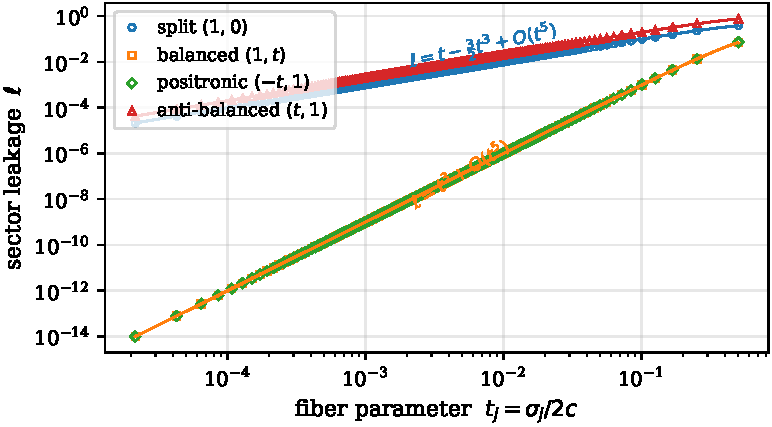
\includegraphics[width=0.92\linewidth]{figures/figT_leakage.pdf}
\caption{Measured per-mode sector leakages of the four trial families
in a $240$-function Laguerre discretization of the $\kappa=-1$ channel
(symbols; one point per SVD fiber), overlaid with the parameter-free
laws of Theorem~\ref{thm:leakage} (lines). The balanced and positronic
families coincide, as the theorem states; agreement is at machine
precision over fourteen decades.}
\label{fig:leakage}
\end{figure}

Figure~\ref{fig:leakage} shows the four laws against the measured
leakages in the actual Laguerre discretization: the reduction is exact
in the discrete setting, so the agreement is limited only by machine
precision. Theorem~\ref{thm:leakage} quantifies the geometry behind
kinetic balance: the balanced constructions are conforming to
\emph{third} order in $t$, the split and anti-balanced ones only to
first order, with the anti-balanced constant twice the split one --- and
this discriminates the sign convention of the dual-balance
family~\cite{Shabaev2004}, whose flipped variant is anti-balanced.

\section{The global conformity defect}\label{sec:defect}

\begin{theorem}[exact global defect]\label{thm:defect}
Let $Q$ have orthonormal columns spanning an untruncated single-family
trial space (one direction of \eqref{eq:families} per fiber), let
$\Pi=QQ^{T}$, and let
$\delta=\norm{(I-\Pi)\Lambda_{+}\Pi}_{2}$. Then, exactly,
\begin{equation}
\delta=\max_{j}\ \ell_{j}\sqrt{1-\ell_{j}^{2}},
\end{equation}
with $\ell_{j}$ the corresponding leakage of
Theorem~\ref{thm:leakage}, and the same value is obtained with
$\Lambda_{-}$ in place of $\Lambda_{+}$.
\end{theorem}

\begin{proof}
$\Pi$, $\Lambda_{\pm}$ and hence $(I-\Pi)\Lambda_{+}\Pi$ are
block-diagonal with respect to the fiber decomposition of
Proposition~\ref{prop:fiber}, and the norm of a block-diagonal matrix
is the maximum of the block norms. On a fiber with unit trial vector
$b$ and $g=\ip{v_{+}}{b}$, one computes
$(I-bb^{T})\,v_{+}v_{+}^{T}\,b=g\,(v_{+}-gb)$, whose squared norm is
$g^{2}(1-2g^{2}+g^{2})=g^{2}(1-g^{2})$ using $\norm{v_{+}}=\norm{b}=1$.
Since $\ip{v_{+}}{b}^{2}+\ip{v_{-}}{b}^{2}=1$ in the fiber,
$g^{2}=1-\ell^{2}$ and the block norm is $\ell\sqrt{1-\ell^{2}}$; the
expression is symmetric under $\ell^{2}\leftrightarrow1-\ell^{2}$,
which proves the $\Lambda_{-}$ statement.
\end{proof}

\begin{corollary}[exact conformity of the dual-balance pair space]
\label{cor:dkb}
The untruncated dual-kinetic-balance pair space, spanned by both
$(1,t_{j})$ and $(-t_{j},1)$ in every fiber, satisfies
$(I-\Pi)\Lambda_{\pm}\Pi=0$ exactly.
\end{corollary}

\begin{proof}
The two directions span each two-dimensional fiber, so $\Pi$ restricts
to the identity on every fiber, and $\Lambda_{\pm}$ preserve fibers.
\end{proof}

Corollary~\ref{cor:dkb} sharpens the empirical picture of dual kinetic
balance: the prescription itself is \emph{exactly} conforming to the
free splitting; any nonzero defect observed in practice is entirely an
effect of truncating the family, and it grows with the basis size only
because the largest singular value does --- in the Laguerre families
used here, $\sigma_{\max}\approx0.64\,\beta N$ (measured exponent
$0.992$), so the danger fibers $t=O(1)$ are always the highest modes.

\section{A pollution dichotomy for bounded potentials}
\label{sec:dichotomy}

For a bounded potential the entire pollution question for single-family
prescriptions reduces to the position of the free Rayleigh values.

\begin{theorem}[pollution dichotomy]\label{thm:dichotomy}
Let $V_{d}\in\R^{N\times N}$ be symmetric with
$\norm{V_{d}}_{2}\le v$ --- in particular the compression of a bounded
multiplication operator with $\norm{V}_{\infty}\le v$ onto the
orthonormal family --- and let $W=\mathrm{diag}(V_{d},V_{d})$. Write
$G_{v}=(-c^{2}+v,\,c^{2}-v)$ and, per fiber,
\begin{equation}
R_{\mathrm{bal}}=c^{2}\frac{1+3t^{2}}{1+t^{2}},\quad
R_{\mathrm{spl}}=c^{2},\quad
R_{\mathrm{pos}}=-R_{\mathrm{bal}},\quad
R_{\mathrm{anti}}=c^{2}\frac{5t^{2}-1}{1+t^{2}}.
\label{eq:rayleigh}
\end{equation}
Then:
\begin{enumerate}
\item[(a)] $R_{\mathrm{bal}}-c^{2}=2c^{2}t^{2}/(1+t^{2})\ge0$;
$R_{\mathrm{anti}}$ lies strictly inside $(-c^{2},c^{2})$ for all
$0<t<1/\sqrt{2}$ and equals the exact gap midpoint $0$ at
$t=1/\sqrt{5}$.
\item[(b)] $\mathrm{spec}(H_{0}+W)\cap G_{v}=\emptyset$.
\item[(c)] Every Galerkin eigenvalue of $H_{0}+W$ on the balanced
family is $\ge c^{2}-v$; on the positronic family, $\le -c^{2}+v$; on
the split family, within $v$ of $c^{2}$. None of these prescriptions
produces an eigenvalue in $G_{v}$, for any bounded potential and with
no smallness condition.
\item[(d)] On the anti-balanced family the sorted Galerkin eigenvalues
lie within $v$ of the sorted $R_{\mathrm{anti}}(t_{j})$; every fiber
with $|R_{\mathrm{anti}}(t_{j})|<c^{2}-2v$ therefore forces a Galerkin
eigenvalue inside $G_{v}$, where by (b) the parent matrix has no
spectrum: a genuine spurious eigenvalue, with predicted location.
\end{enumerate}
\end{theorem}

\begin{proof}
(a) is direct computation from \eqref{eq:rayleigh}:
$c^{2}-R_{\mathrm{anti}}=c^{2}(2-4t^{2})/(1+t^{2})$ and
$R_{\mathrm{anti}}+c^{2}=6c^{2}t^{2}/(1+t^{2})$.
For a matrix $Q$ with orthonormal columns,
$\norm{Q^{T}WQ}\le\norm{W}=\norm{V_{d}}\le v$ (Cauchy--Schwarz on unit
vectors $Qx$), and for the compression of a multiplication operator
$\norm{V_{d}}\le\norm{V}_{\infty}$ by the same argument in $L^{2}$.
$Q^{T}H_{0}Q$ is diagonal with entries \eqref{eq:rayleigh} by
Proposition~\ref{prop:fiber} and the proof of
Theorem~\ref{thm:defect}. Weyl's eigenvalue perturbation inequality,
$|\lambda_{k}(D+P)-\lambda_{k}(D)|\le\norm{P}$ for symmetric matrices,
applied with $D=H_{0}$, $P=W$ gives (b), since
$\mathrm{spec}(H_{0})=\{\pm E(\sigma_{j})\}$ avoids $(-c^{2},c^{2})$;
applied with $D=Q^{T}H_{0}Q$, $P=Q^{T}WQ$ it gives (c) and the pairing
in (d). If $|R_{\mathrm{anti}}(t_{j})|<c^{2}-2v$ the paired eigenvalue
$e$ satisfies $|e|\le|R_{\mathrm{anti}}|+v<c^{2}-v$, so $e\in G_{v}$.
\end{proof}

\begin{remark}
Part (d) explains the classical wrong-sign pathology quantitatively:
the anti-balanced direction \emph{sweeps the gap}, its free Rayleigh
value traversing all of $(-c^{2},c^{2})$ as $t$ runs over
$(0,1/\sqrt{2})$. The physical dual-balance sign of
Ref.~\cite{Shabaev2004} is precisely the choice that avoids this sweep.
The classical spurious states of equal-basis discretizations at
$\kappa>0$~\cite{DrakeGoldman1981,Pestka2003}, exactly degenerate with
the $-\kappa$ ground state~\cite{Tupitsyn2008}, are a distinct,
Coulomb-specific phenomenon outside the scope of
Theorem~\ref{thm:dichotomy}; in the companion discretization they are
reproduced at the $10^{-13}$ level~\cite{companion}.
\end{remark}

\section{The cusp lemma}\label{sec:cusp}

The point-nucleus Coulomb--Dirac eigenfunctions carry the prefactor
$r^{\gamma}$, $\gamma=\sqrt{\kappa^{2}-(Z/c)^{2}}$. Consider the
orthonormal generalized Laguerre family with prefactor power $\mu$,
\begin{equation}
q_{j}^{(\mu)}(x)=\sqrt{\frac{j!}{\Gamma(j+2\mu+1)}}\;
x^{\mu}e^{-x/2}L_{j}^{(2\mu)}(x).
\label{eq:qj}
\end{equation}

\begin{theorem}[exact representation]\label{thm:exact}
For $\kappa<0$ the lowest point-nucleus state of channel $\kappa$ has
both components proportional to the same profile
$r^{\gamma}e^{-(Z/|\kappa|)r}$, with eigenvalue
$E=\gamma c^{2}/|\kappa|$. Consequently, in the basis \eqref{eq:qj}
with $\mu=\gamma$ and scale matched to $Z/|\kappa|$, the ground state
lies in the span of $q_{0}^{(\gamma)}$ alone: the discretized problem
reproduces it exactly with two degrees of freedom.
\end{theorem}

\begin{proof}
Insert the ansatz $(a,b)\,r^{\gamma}e^{-\lambda r}$ into
$h_{\kappa}\psi=E\psi$ with $V=-Z/r$. Each row produces one condition
proportional to $r^{\gamma-1}$ and one to $r^{\gamma}$; the four
conditions are linear in $(a,b)$ and consistent precisely when
$\lambda=Z/|\kappa|$ and $E=\gamma c^{2}/|\kappa|$, with a unique ratio
$b/a$ (for $\kappa=-1$, $b/a=Z/(c(\kappa-\gamma))$). The state is
nodeless and matches the $n_{r}=0$ entry of the Sommerfeld spectrum,
hence is the ground state of the channel. Since
$r^{\gamma}e^{-\lambda r}\propto q_{0}^{(\gamma)}(2\lambda r)$, both
components lie in the one-dimensional span of $q_{0}^{(\gamma)}$.
\end{proof}

In the certified implementation this is observed literally: the
two-degree-of-freedom discretization reproduces the ground binding
energy of $Z$ up to $130$ at relative accuracy
$10^{-15}$~\cite{companion}.

\begin{theorem}[universal rate dichotomy]\label{thm:rate}
Let $u(x)=x^{\gamma}e^{-x/2}$ with $\gamma>0$, and let
$c_{j}=\ip{q_{j}^{(\mu)}}{u}$, $\mu>0$. Then, exactly,
\begin{equation}
c_{j}=\sqrt{\frac{j!}{\Gamma(j+2\mu+1)}}\;
\frac{\Gamma(\mu+\gamma+1)\,\Gamma(j+\mu-\gamma)}
{j!\;\Gamma(\mu-\gamma)},
\label{eq:coef}
\end{equation}
so that
$|c_{j}|\sim\bigl[\Gamma(\mu+\gamma+1)/|\Gamma(\mu-\gamma)|\bigr]\,
j^{-(1+\gamma)}$ as $j\to\infty$. In particular:
\begin{enumerate}
\item[(a)] the decay exponent $-(1+\gamma)$ is independent of $\mu$;
a mismatched prefactor improves only the constant, never the rate;
\item[(b)] $c_{j}=0$ for all $j\ge1$ if and only if
$\mu-\gamma\in\{0,-1,-2,\dots\}$; in particular the matched basis
$\mu=\gamma$ represents $u$ exactly;
\item[(c)] the $L^{2}$ tail after $N$ terms scales as
$N^{-(1/2+\gamma)}$.
\end{enumerate}
\end{theorem}

\begin{proof}
Formula \eqref{eq:coef} follows from the classical integral
$\int_{0}^{\infty}e^{-x}x^{s}L_{j}^{(\alpha)}(x)\,dx=
\Gamma(s+1)\Gamma(j+\alpha-s)/(j!\,\Gamma(\alpha-s))$ with
$s=\mu+\gamma$, $\alpha=2\mu$. The asymptotics follow from
$\Gamma(j+a)/\Gamma(j+b)\sim j^{a-b}$: the normalization contributes
$j^{-\mu}$ and the ratio $\Gamma(j+\mu-\gamma)/j!$ contributes
$j^{\mu-\gamma-1}$, so the $\mu$-dependence cancels in the exponent.
The vanishing condition is the pole condition of
$1/\Gamma(\mu-\gamma)$ together with positivity of the remaining
factors, and (c) follows by summing $|c_{j}|^{2}\sim j^{-2-2\gamma}$.
\end{proof}

Theorem~\ref{thm:rate} is the approximation-theoretic content of
``exact structure or nothing'': adaptive approximation of the cusp with
any prefactor other than $\gamma$ itself faces the fixed algebraic rate
$N^{-(1/2+\gamma)}$ in norm, no matter how the prefactor is tuned. This
is consistent with, and explains, the operating accuracies of recent
adaptive spectral solvers~\cite{ChenShaoWu2026} as compared with the
matched-basis solver of the companion paper~\cite{companion}. The
formula \eqref{eq:coef} is verified at quadrature precision
($10^{-9}$) across $\mu\in\{0.9,1,2\}$, the measured constant ratios
agree with $\Gamma(\mu+\gamma+1)/|\Gamma(\mu-\gamma)|$ to five digits,
and the measured decay slopes converge monotonically to
$-(1+\gamma)$~\cite{companion}.

\section{Numerical evidence at the Coulomb frontier}
\label{sec:frontier}

Three measured facts delimit what remains to be proven. All were
obtained with the certified discretization of~\cite{companion}
(run-time verification of the assembly identities; exact quadrature at
the matched prefactor).

\emph{(i) Eigenvalue rate.} For mismatched bases the ground-state
eigenvalue error decays as $N^{-2\gamma}$: measured exponents
$-1.901/-1.605/-0.928$ against $2\gamma=1.913/1.624/0.966$ at
$Z=40/80/120$ ($\kappa=-1$, integer prefactor), with a
\emph{fractional} mismatched prefactor $\mu=\gamma+0.3$ giving the same
exponent ($-1.593$) at a different constant, exactly as
Theorem~\ref{thm:rate}(a) demands. The mechanism is quadratic in the
form norm: the measured ratio
$|\delta E_{N}|/\ip{r_{N}}{|H_{0}|\,r_{N}}$, with $r_{N}$ the
projection residual of the exact eigenfunction, is $0.43$--$0.55$ over
the trustworthy window.

\begin{conjecture}[first-order dual estimate]\label{conj:dual}
For the Galerkin approximation of an isolated eigenvalue of
$h_{\kappa}$ from a conforming family,
$|\delta E_{N}|\le C\,\ip{r_{N}}{|H_{0}|\,r_{N}}$ with $C$ of order
unity; combined with Theorem~\ref{thm:rate} this yields the
$N^{-2\gamma}$ law.
\end{conjecture}

\emph{(ii) Relative bounds.} The operator-norm relative bound
$\norm{W H_{0}^{-1}}$ and the form bound
$\norm{\,|H_{0}|^{-1/2}W|H_{0}|^{-1/2}}$ of the discretized Coulomb
potential \emph{diverge} with $N$ ($\sim N^{0.46}$ and $\sim\log N$
respectively): no Kato--Hardy inequality can hold uniformly relative to
the \emph{discretized} free operator, because
$(\Pi H_{0}\Pi)^{-1}\ne\Pi H_{0}^{-1}\Pi$ --- the discrete operator caps
the available momentum at $\sigma_{\max}\approx0.64\beta N$ while the
basis keeps resolving the $1/r$ singularity. By contrast, the same form
bound measured against the $|H_{0}|$ of a much larger nested reference
--- a proxy for the continuum operator --- \emph{converges} (e.g.\
$0.8633\to0.8687$ at $Z=92$ with halving increments), remaining below
$1$ up to $Z/c\approx0.75$ at practical basis sizes.

\begin{conjecture}[continuum-relative protection]\label{conj:coulomb}
Formulated with the spectral projectors and the absolute value of the
\emph{continuum} free operator, the protection statement of
Theorem~\ref{thm:dichotomy}(c) extends to the point-Coulomb potential
for the balanced families in the matched basis, in the coupling range
where the continuum-relative form bound is smaller than the fiber
Rayleigh margin. The divergence of the discrete-relative bounds shows
that no proof can proceed relative to the discretized free operator;
compressions in the sense of Lewin--S\'er\'e~\cite{LewinSere2010} are
necessary.
\end{conjecture}

\emph{(iii) The impostor's trajectory.} At point Coulomb coupling the
anti-balanced (sign-flipped dual-balance) discretization carries a
spurious gap eigenvalue already at the smallest basis sizes and at
every $Z$ tested: it is born at the \emph{lower} gap edge (binding
$-36905$ at $Z=1$, $N=20$, i.e.\ $E\approx-0.965\,c^{2}$) and dives
toward the gap midpoint as $N$ grows ($-36905\to-28314$ for
$N=20\to80$) --- the sweep of $R_{\mathrm{anti}}$ of
Theorem~\ref{thm:dichotomy}(d) made visible, accelerated by the
unbounded potential. Matching this trajectory quantitatively is the
natural sharpness test for Conjecture~\ref{conj:coulomb}.

\section{A conditional exclusion window at Coulomb coupling}
\label{sec:t1c}

The measured constants of Section~\ref{sec:frontier} support a
finite-dimensional exclusion theorem at point Coulomb coupling. Split
the fibers at $t^{*}$ into a low sector $L$ ($t_{j}\le t^{*}$) and a
high sector $H$ ($t_{j}>t^{*}$), write $D^{*}=\sqrt{1+4t^{*2}}$, and
let $E_{L},E_{H}$ denote the fiber energies on the full pair spans of
each sector. Suppose the discretized Coulomb form satisfies the
measured bounds
$\norm{E_{L}^{-1/2}W_{LL}E_{L}^{-1/2}}\le\omega_{L}$,
$\norm{E_{L}^{-1/2}W_{LH}E_{H}^{-1/2}}\le x$, and
$\norm{E_{H}^{-1/2}W_{HH}E_{H}^{-1/2}}\le\omega_{H}$.

\begin{theorem}[conditional exclusion window]\label{thm:t1c}
Let $\rho_{H}(m)=D^{*}c^{2}/(D^{*}c^{2}-m)$ and suppose
$\omega_{H}\rho_{H}(m)<1$ and
\[
\Bigl[\omega_{L}
+\frac{x^{2}\rho_{H}(m)}{1-\omega_{H}\rho_{H}(m)}\Bigr]
\frac{c^{2}}{c^{2}-m}<1 .
\]
Then the full pair-space Galerkin matrix of $h=H_{0}+W$ has no
eigenvalue $E$ with $|E|<m$.
\end{theorem}

\begin{proof}
On the high sector $|h_{H}|\ge D^{*}c^{2}$, so
$\norm{E_{H}^{1/2}(h_{H}-\mu)^{-1}E_{H}^{1/2}}\le\rho_{H}(m)$ for
$|\mu|\le m$ (the function $E/(E-m)$ decreases in $E$ on the spectrum);
with the $\omega_{H}$ bound and a Neumann series,
$h_{H}+W_{HH}-\mu$ is invertible with weighted resolvent bound
$\rho_{H}/(1-\omega_{H}\rho_{H})$. The Schur complement onto $L$ then
carries a correction of weighted norm at most
$x^{2}\rho_{H}/(1-\omega_{H}\rho_{H})$, while
$\norm{E_{L}^{1/2}(h_{L}-\mu)^{-1}E_{L}^{1/2}}\le c^{2}/(c^{2}-m)$
since $E_{j}\ge c^{2}$ on $L$. The displayed condition makes the Schur
complement invertible, and the Feshbach block lemma yields
invertibility of the full pencil at every $|\mu|<m$.
\end{proof}

At $Z=40$ ($\nu=0.29$, $t^{*}=1$) the measured constants
$(\omega_{L},\omega_{H},x)=(0.19,0.35,0.20)$ give
$m^{*}\approx0.70\,c^{2}$: the theorem excludes eigenvalues from the
deep two-thirds of the upper gap, the physical ladder (which starts at
$\gamma c^{2}=0.96\,c^{2}$) sits above the window, and the certified
solver spectrum is verified to contain no eigenvalue inside it. This
is, to our knowledge, the first quantitative pollution-exclusion window
for a point-Coulomb Dirac discretization. At strong coupling
($Z\gtrsim90$) the two-sector hypothesis fails through $\omega_{H}$:
the measured dyadic scale decomposition shows bounded within-scale
blocks ($\Omega_{kk}\approx0.35$--$0.57$, stable under basis growth)
but flat cross-scale couplings ($\approx0.2$ between \emph{all} scale
pairs --- the scale invariance of $1/r$ in action), so the row sums
grow logarithmically. Beating this flat cross-scale structure with a
multi-scale (Littlewood--Paley-type) elimination, using the analytic
structure of the relativistic Hardy inequality rather than norm bounds
alone, is the precisely delimited remaining step toward the
unconditional theorem.

\section{Concluding remarks}

The fiber reduction turns kinetic-balance pollution from an observed
phenomenon into computable algebra: exact leakage laws with exponents
$3/1/3/1$ and constants $1/1/1/2$, an exact global defect, exact
conformity of the untruncated dual-balance pair space, and a pollution
dichotomy for bounded potentials in which the protected window and the
locations of the guaranteed impostors are explicit. The cusp lemma
supplies the complementary approximation statement with a universal
exponent. What separates this elementary picture from the full
point-Coulomb theorem is precisely quantified --- and measured: the
failure of discrete-relative bounds, the convergence of
continuum-relative ones, and the impostor trajectory that any complete
theory must reproduce. All numerical statements are reproducible from
the open verification scripts accompanying the companion
paper~\cite{companion}, and the core algebraic identities of
Theorems~\ref{thm:leakage}, \ref{thm:defect} and~\ref{thm:dichotomy}(a)
--- the balanced-leakage identity $t-\rho=4t^{3}/(1+w)^{2}$, the
per-fiber defect $g^{2}(1-g^{2})$, and the in-gap characterization of
the anti-balanced Rayleigh value with its mid-gap crossing at
$t=1/\sqrt{5}$ --- have additionally been machine-verified in Lean~4
with Mathlib; the proof files accompany the repository.

\begin{thebibliography}{99}

\bibitem{Talman1986} J.~D. Talman,
\emph{Minimax principle for the Dirac equation},
Phys. Rev. Lett. \textbf{57}, 1091 (1986).

\bibitem{DES2000} J.~Dolbeault, M.~J. Esteban, and E.~S\'er\'e,
\emph{On the eigenvalues of operators with gaps. Application to Dirac
operators}, J. Funct. Anal. \textbf{174}, 208 (2000).

\bibitem{MorozovMuller2015} S.~Morozov and D.~M\"uller,
\emph{On the minimax principle for Coulomb--Dirac operators},
Math. Z. \textbf{280}, 733 (2015).

\bibitem{LewinSere2010} M.~Lewin and E.~S\'er\'e,
\emph{Spectral pollution and how to avoid it},
Proc. London Math. Soc. \textbf{100}, 864 (2010).

\bibitem{LevitinShargorodsky2004} M.~Levitin and E.~Shargorodsky,
\emph{Spectral pollution and second-order relative spectra for
self-adjoint operators}, IMA J. Numer. Anal. \textbf{24}, 393 (2004).

\bibitem{Shabaev2004} V.~M. Shabaev, I.~I. Tupitsyn, V.~A. Yerokhin,
G.~Plunien, and G.~Soff,
\emph{Dual kinetic balance approach to basis-set expansions for the
Dirac equation}, Phys. Rev. Lett. \textbf{93}, 130405 (2004).

\bibitem{Grant2007} I.~P. Grant,
\emph{Relativistic Quantum Theory of Atoms and Molecules}
(Springer, New York, 2007).

\bibitem{Kutzelnigg1984} W.~Kutzelnigg,
\emph{Basis set expansion of the Dirac operator without variational
collapse}, Int. J. Quantum Chem. \textbf{25}, 107 (1984).

\bibitem{DrakeGoldman1981} G.~W.~F. Drake and S.~P. Goldman,
\emph{Application of discrete-basis-set methods to the Dirac equation},
Phys. Rev. A \textbf{23}, 2093 (1981).

\bibitem{Pestka2003} G.~Pestka,
\emph{Spurious roots in the algebraic Dirac equation},
Phys. Scr. \textbf{68}, 254 (2003).

\bibitem{Tupitsyn2008} I.~I. Tupitsyn and V.~M. Shabaev,
\emph{Spurious states of the Dirac equation in a finite basis set},
Opt. Spectrosc. \textbf{105}, 183 (2008).

\bibitem{ChenShaoWu2026} J.~Chen, S.~Shao, and H.~Wu,
\emph{An adaptive log-orthogonal spectral method for the radial Dirac
eigenvalue problem}, arXiv:2604.11063 [math.NA] (2026).

\bibitem{companion} C.~D. Reinoso,
\emph{Exact-structure spectral discretization of the point-nucleus
radial Dirac equation}, companion paper (2026).

\end{thebibliography}

\end{document}
